\documentclass[12pt]{article}
\usepackage{fullpage}
\usepackage{amsmath}
\usepackage{hyperref}
\usepackage{graphicx}
\usepackage{listings}
\usepackage{float}
\usepackage{}

\floatstyle{plain}
\newfloat{snippet}{thb}{lop}
\floatname{snippet}{Snippet}


\begin{document}
  \begin{center}
    \textbf{\large Out-of-Order SMIPS} \\
    6.375 Microarchitecture Design Proposal\\
    6 April 2011 \\
    
    \vspace{\baselineskip}
    
    \emph{Team}: David S. Greenberg and Bhaskar Mookerji
  \end{center}

For our 6.375 final project, we are implementing a superscalar processor using Tomasulo's algorithm.

\section{Microarchitecture Overview}

\begin{figure}[ht!]
    \centering
    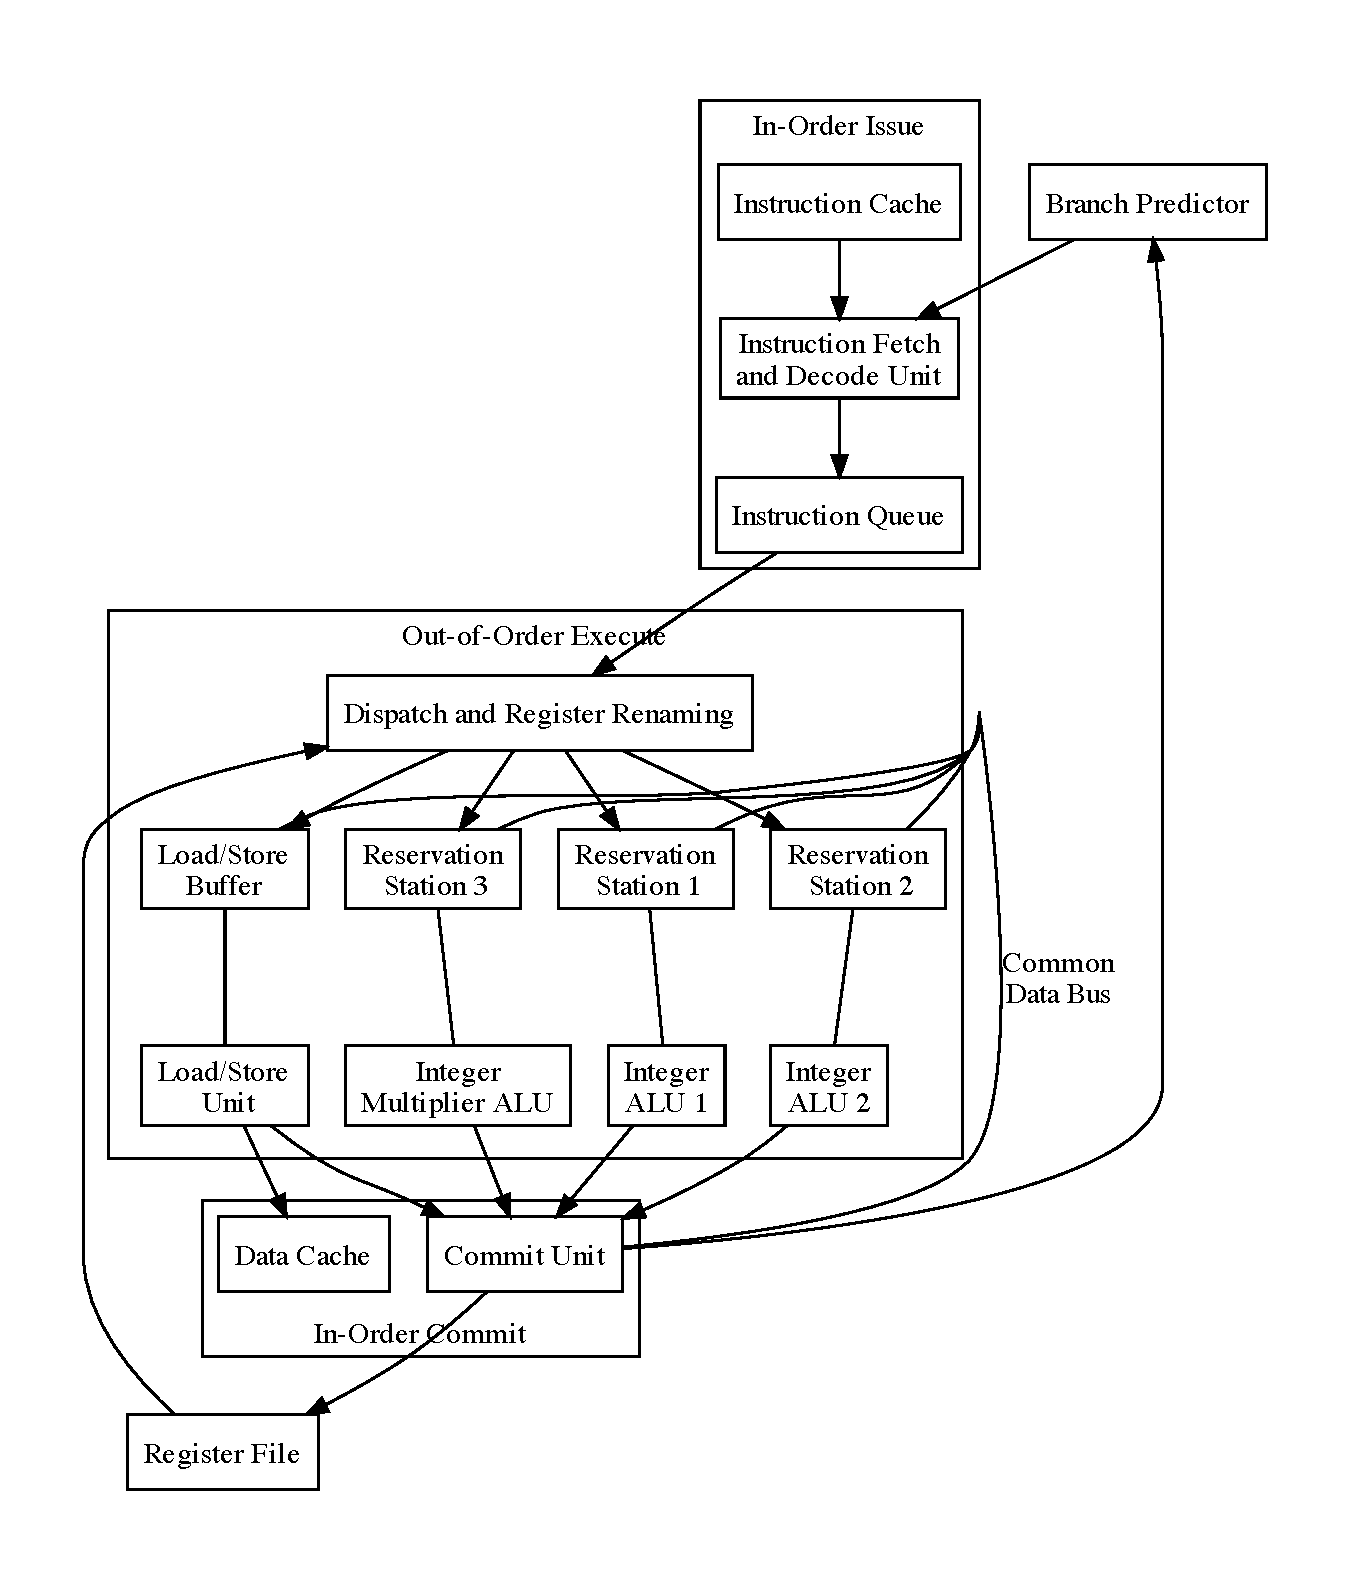
\includegraphics[width=\textwidth]{figures/design.pdf}
    \caption{System architecture using out-of-order execution and pipelined integer arthmetic. \label{fig:design}}
\end{figure}

\begin{figure}[h]
    \centering
    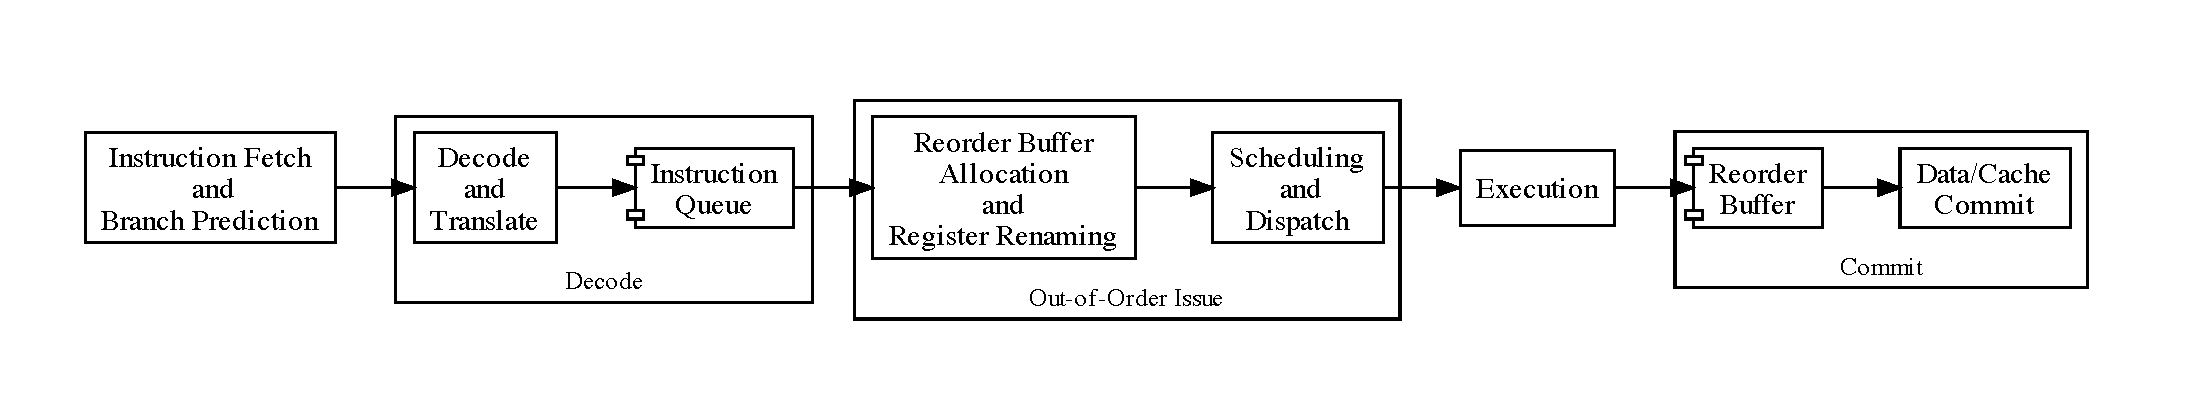
\includegraphics[width=1.1\textwidth]{figures/pipeline.pdf}
    \caption{Instruction pipeline. Pipeline stage is labeled in-box, unless superseded by an overbox. A component box indicates component (such as a FIFO) between stages. Not included in this diagram is the reservation stations and load/store buffer in the execution stage.\label{fig:pipeline}}
\end{figure}

\subsection{New System Types}

\begin{enumerate}
    \item \textbf{Reorder Buffer Token}
This is used to know which instruction (and thus its destination register) some piece of data corresponds to (could be an instruction or a result)
    \item \textbf{Reservation Station Entries}
Stores the reorder token it corresponds to, the operation to execute, and either the computed operands or the token that will contain their result.
    \item \textbf{Reorder Buffer Entries}
For ALU ops, stores the destination register, the Maybe#(value), and the epoch of the instruction.
For branch ops, stores the same stuff as the ALU ops AND, if it was a mispredict, the correct address.
    \item \textbf{Common Data Bus format}
The CDB has the ROB token, value, and the Maybe#(mispredict)
\end{enumerate}

\section{Pipeline Stage Interfaces}

\begin{enumerate}
    \item \textbf{Pipeline Container: Processor}
    \item \textbf{Instruction Fetch}
    \item \textbf{Instruction Decode and Dispatch}
    \item \textbf{Execute}
    \item \textbf{Writeback and Commit}
\end{enumerate}

\section{Architectural Interfaces}

\begin{enumerate}
    \item \textbf{Issue and Dispatch Units}
Inputs: instruction fifo
Outputs: Reservation Station Entry fifos to the various execute units' reservation stations
Uses: ROB token request/entry placement

Other side effects: updates the register map with the ROB token

rules: if ROB token available and instruction ready, unpack the instruction, fill in the known operands, send to a reservation station
if the instruction is a store, instead wait for ROB to empty and then issue it
    \item \textbf{Reservation Stations}
Inputs: reservation station entry fifo
Outputs: send instruction to execute unit

rules: snooping CDB and updating operands of held entries until they're ready
issuing intructions when they're ready
    \item \textbf{Common Data Bus}
Inputs: execution result (put with method Action)
Outputs: execution result (multiple reader get (fanout))

invariant: all listeners must check the bus every cycle and never drop a packet

Potential impl: bypass reg storing value, every listener must ack before accepting a new value
    \item \textbf{Reorder Buffer}
inputs: listening to CDB, side effects of token requests
outputs: none

rules: graduate last instruction if it's been computed (includes writeback and removal from circular buffer)
purge instructions of wrong epoch
issue a mispredict if a branch had been mispredicted

Other side effects: update the register map to use the architectural register for map entries whose token matches graduated instruction
    \item \textbf{Branch Predictor}
It's a BTB
Has a function that tells what it would predict given its current state
Has a function to speculate the next instruction
Has a function to tell it that it mispredicted and needs to fix it
Has a function to tell what epoch it is

    \item \textbf{Execute unit}
Must transparent pass reorder token so that it can be bypassed correctly
\end{enumerate}
    
\section{Goals and Testing Strategy}

\subsection{Functional Correctness}
We'll add 0-2 cycle latencies to all instructions in the pipeline. Then, we collect IPC benchmarks with the added latencies.
Next, we collect benchmarks with Tomasulo's algorithm enabled. We should see a significant improvement due to the latencies
being hidden.
\subsection{FPGA Synthesis}
We've removed all CAM from the system, and so we believe that we should be able to synthesize modulo routing constraints.
\subsection{Performance}
Raw performance is not the goal of this project. Rather, theoretical performance and correctness are the primary concerns.
Our design should enable future developers to use a modularized Tomasulo's algorithm to hide the latencies of their additional instructions.
Unfortunately, there is way to show a strict benefit to the elastic pipelined SMIPS processor, since all ALU ops and multiplies 
are single cycle on an FPGA anyway, and any worthwhile multicycle op is a project in and of itself to implement. Bam.

 \end{document}
